
% This LaTeX was auto-generated from MATLAB code.
% To make changes, update the MATLAB code and republish this document.

\documentclass{article}
\usepackage{graphicx}
\usepackage{geometry}
\geometry{a4paper, portrait, margin=.5in}
\usepackage{color}


\sloppy
\definecolor{lightgray}{gray}{0.5}
\setlength{\parindent}{0pt}

\begin{document}
	
	
	
	\section*{OCT Project - Ashley Clark}
	
	
	\subsection*{Contents}
	
	\begin{itemize}
		\setlength{\itemsep}{-1ex}
		\item Foveal Pit Contour Algorithm - Dubis et al 2009
		\item Anatomical Landmarks Algorithm - Dubis et al 2009
		\item Anatomical Landmarks Figure - Dubis et al 2009
		\item Current Crowding Subjects
	\end{itemize}
	
	
	\subsection*{Foveal Pit Contour Algorithm - Dubis et al 2009}
	
	\begin{par}
		"We tested several functions for their ability to fit foveal pit contour,and found that a difference of Gaussians (DoG) function (equation 1) provides the best fit to the foveal OCT scans".
	\end{par} \vspace{1em}
	\begin{par}
		
		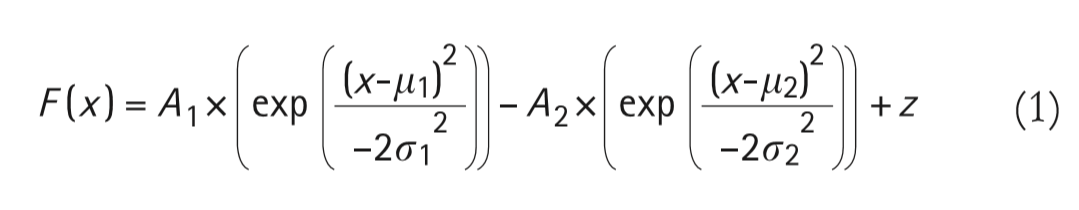
\includegraphics [width=4in]{PitEquation.png}
		
	\end{par} \vspace{1em}
	\begin{par}
		"One of the problems with reconstructing foveal volumes from time-domain OCT is eye movement. Even in individuals with superior fixation stability, small saccades occur that can disrupt the ability to automatically model the pit contour. Thus, aligning scans from within the fast mac data set is an important first step in reconstructing foveal morphology. Using the DoG mean (\$\ensuremath{\backslash}mu\$1 and \$\ensuremath{\backslash}mu\$2 in equation 1), we approximate the lateral shift for each scan, relative to an arbitrary center."
	\end{par} \vspace{1em}
	
	
	\subsection*{Anatomical Landmarks Algorithm - Dubis et al 2009}
	
	\begin{par}
		"To identify anatomical landmarks within the scan, we examine the first derivative F9(x) of the DoG fit".
	\end{par} \vspace{1em}
	\begin{par}
		
		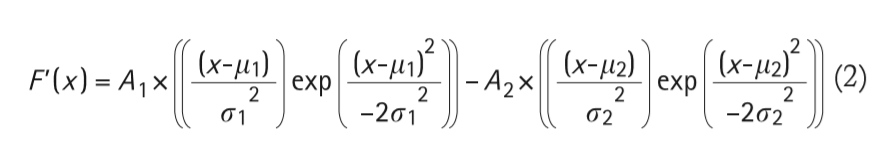
\includegraphics [width=4in]{AnatomyEquation.png}
		
	\end{par} \vspace{1em}
	
	
	\subsection*{Anatomical Landmarks Figure - Dubis et al 2009}
	
	\begin{par}
		
		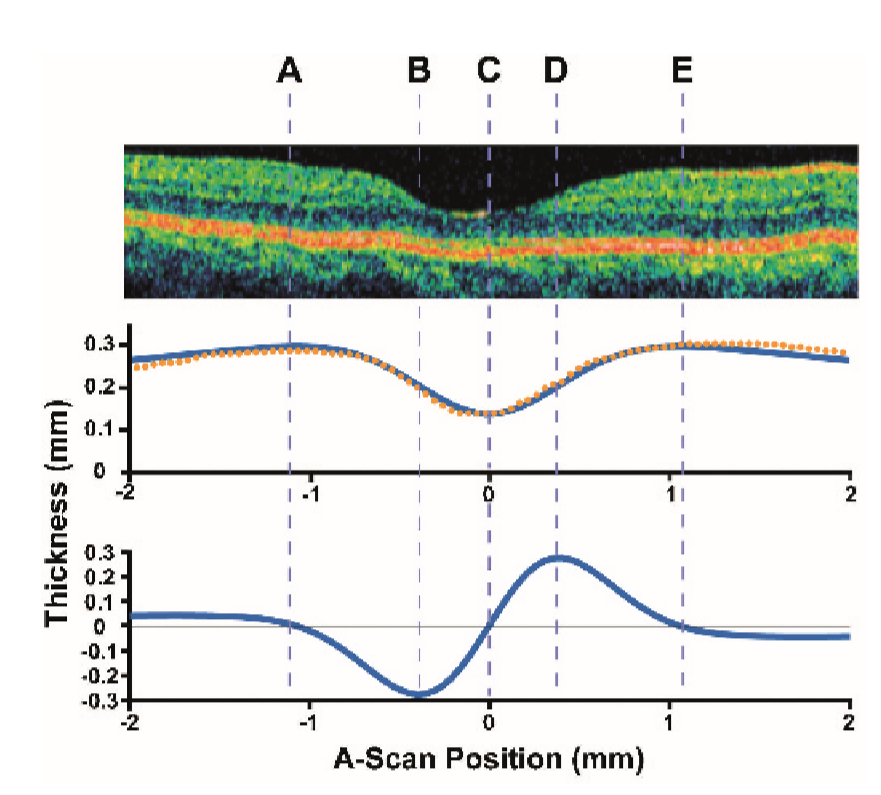
\includegraphics [width=4in]{AnatomyFigure.png}
		
	\end{par} \vspace{1em}
	\begin{par}
		Foveal parameters are derived from specific locations with in the scan. The top panel shows a 4 mm section of an individual line scan from the Stratus system. The middle panel shows a plot of the raw thickness data for this scan (filled circles) and the difference of Gaussian (DoG) fit to the data (solid line). The bottom panel shows the first derivative of this DoG fit. Drawn through these plots are lines A–E, corresponding to objectively defined anatomical landmarks (see text) From these five landmarks(A-E), we can extract three prominent features of the foveal pit—diameter, depth and slope. We define diameter as the distance from rim to rim**,1 13 illustrated in [this figure] as the distance between points A and E.\_
	\end{par} \vspace{1em}
	\begin{par}
		\textit{Points A and E indicate the peak of the foveal rim, as the slope of the foveal contour is zero at these locations. Likewise, point C has a zero slope, and this marks the centre of the pit.}
	\end{par} \vspace{1em}
	
	
	\subsection*{Current Crowding Subjects}
	
	\begin{par}
		Here are which studies these subjects have participated in. \ensuremath{\backslash}textit\{This information is on a shared excel spreadsheet on OPUS/General/ApLab Subject Info.xlsx
	\end{par} \vspace{1em}
	\begin{verbatim}
	octMeasures = [0.1312,1.5465,17.4411,1.8891,0.0556;...
	0.1329,2.2118,12.0650,3.8685,0.1266;...
	0.1279,2.2340,11.2705,3.9466,0.1337;...
	0.1455,2.1889,13.5556,3.7989,0.1388;...
	0.1051,1.7964,11.5957,2.5579,0.0727;...
	0.0999,1.9508,9.9703,3.0077,0.0875;...
	0.1258,2.0279,12.3012,3.2424,0.1121];
	
	subjects = {'Z023','Ashley','Z064','Z046','Z014','Z002','Z084'};
	colors = jet(length(subjects));
	
	thresholdU = ...
	[1.38792522386685,...
	1.18697683662560,...
	1.62139637607767,...
	1.51225625260600,...
	1.67242319632557,...
	1.43399806258883,...
	1.74632405974870];
	
	spanU = [3.1320553,2.1291687,3.1039777,3.8910327,4.2854223,3.9194658,3.2190833];
	
	thresholdC = [...
	2.11248035136737,...
	1.73744526774839,...
	2.04878360709985,...
	1.90715088625624,...
	1.88712963129020,...
	1.91895246256101,...
	2.31159172690596];
	
	spanC = [3.6056974,2.3294666,3.7646437,3.5776696,4.3793206,3.6877453,3.0503151];
	octNames = {'pitDepth(mm)','pitDiameter(mm)', 'pitSlope', 'pitArea(mm2)', 'pitVolume(mm3)'};
	
	for ii = 1:length(subjects)
	%     for octIdx = 1:length(octNames)
	octPitDepth(ii) = octMeasures(ii,1);
	octPitDiameter(ii) = octMeasures(ii,2);
	octPitSlope(ii)= octMeasures(ii,3);
	octPitArea(ii)= octMeasures(ii,4);
	octPitVolume(ii)= octMeasures(ii,5);
	%     end
	end
	
	
	for octIdx = 1:length(octNames)
	figure;
	
	subplot(2,2,1)
	[~,p,~,r] = LinRegression(thresholdU,octMeasures(:,octIdx)',0,NaN,1,0);
	hold on
	for ii = 1:length(subjects)
	leg(ii) = scatter(thresholdU(ii),octMeasures(ii,octIdx)',100,...
	[colors(ii,1) colors(ii,2) colors(ii,3)],'filled','Linewidth',5);
	end
	xlim([0 4]);
	ylim([min(octMeasures(:,octIdx)) max(octMeasures(:,octIdx))])
	xlabel('Uncrowded Threshold')
	legend(leg,subjects)
	
	subplot(2,2,2)
	[~,p,~,r] = LinRegression(thresholdC,octMeasures(:,octIdx)',0,NaN,1,0);
	hold on
	scatter(thresholdC,octMeasures(:,octIdx)',100,colors,'filled','Linewidth',5);
	ylim([min(octMeasures(:,octIdx)) max(octMeasures(:,octIdx))])
	xlim([0 4]);
	xlabel('Crowded Threshold')
	
	subplot(2,2,3)
	[~,p,~,r] = LinRegression(spanU,octMeasures(:,octIdx)',0,NaN,1,0);
	hold on
	scatter(spanU,octMeasures(:,octIdx)',100,colors,'filled','Linewidth',5);
	ylim([min(octMeasures(:,octIdx)) max(octMeasures(:,octIdx))])
	xlim([0 6])
	xlabel('Uncrowded Span')
	
	subplot(2,2,4)
	[~,p,~,r] = LinRegression(spanC,octMeasures(:,octIdx)',0,NaN,1,0);
	hold on
	scatter(spanC,octMeasures(:,octIdx)',100,colors,'filled','Linewidth',5);
	ylim([min(octMeasures(:,octIdx)) max(octMeasures(:,octIdx))])
	xlim([0 6])
	xlabel('Crowded Span')
	
	suptitle(sprintf('%s',octNames{octIdx}));
	set(gcf,'Position',[2000, 100, 700, 900])
	end
	\end{verbatim}
	
	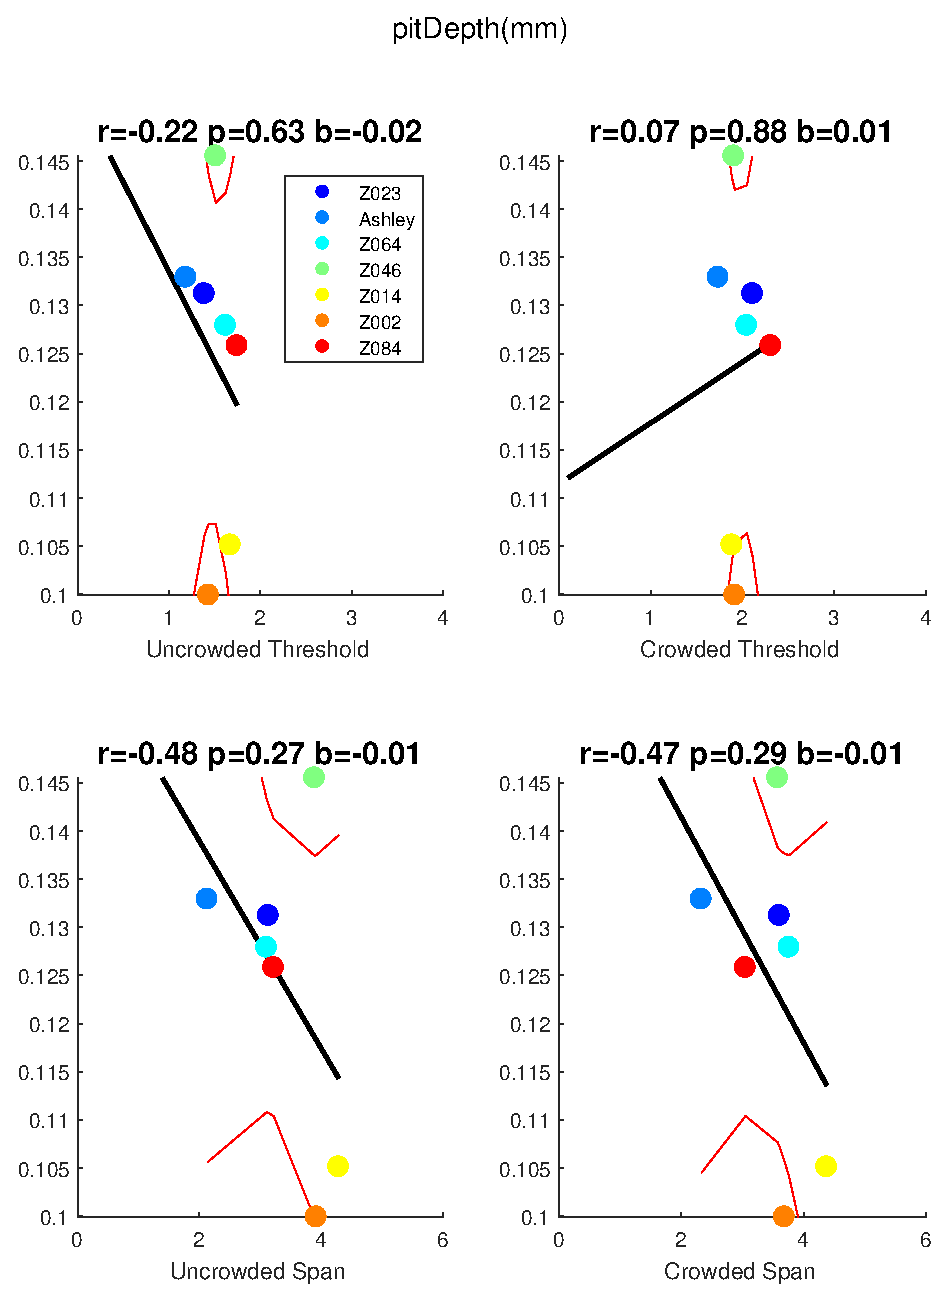
\includegraphics [width=4in]{runOCTAnalysis_01.eps}
	
	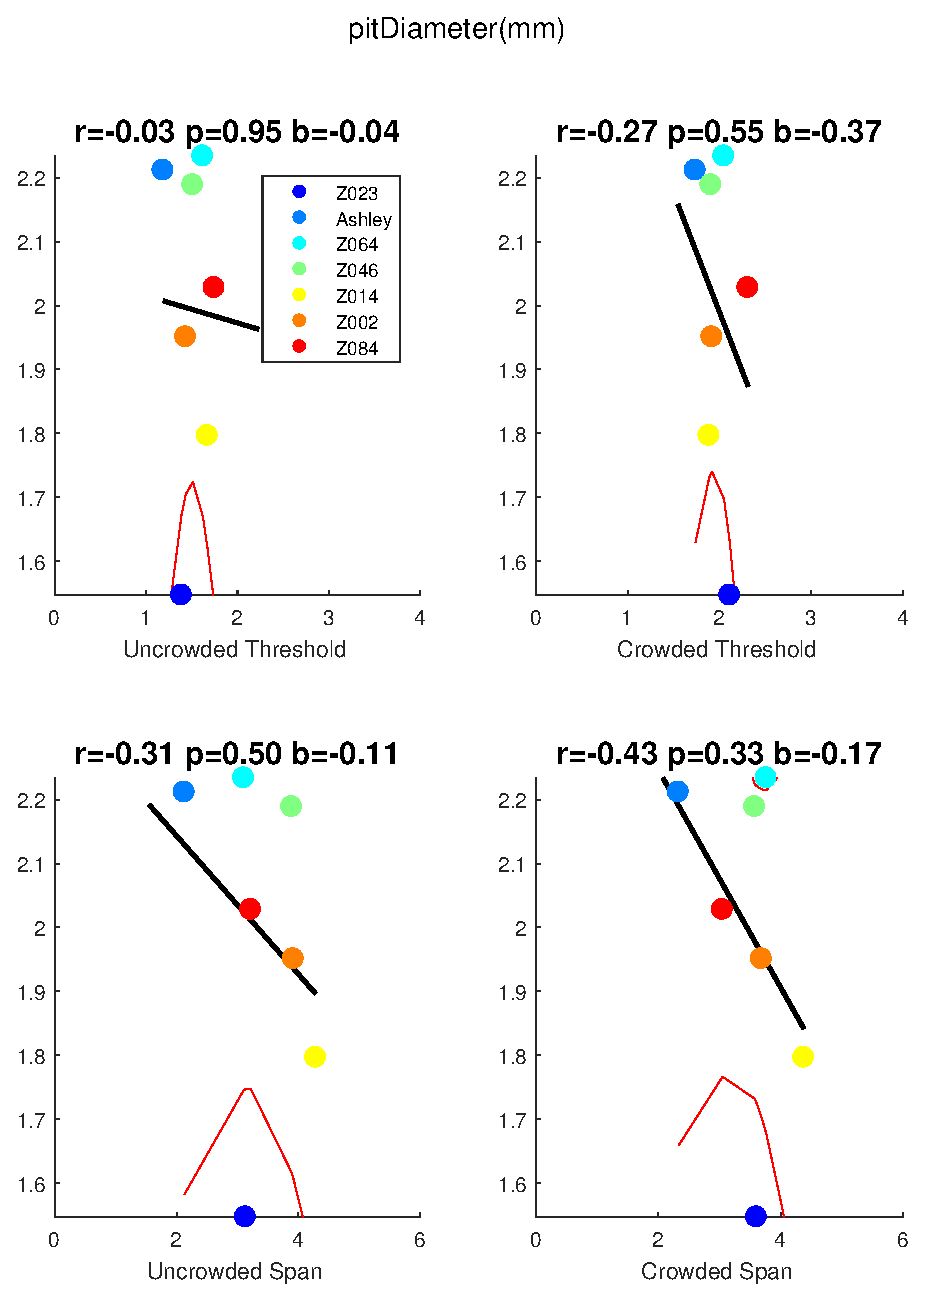
\includegraphics [width=4in]{runOCTAnalysis_02.eps}
	
	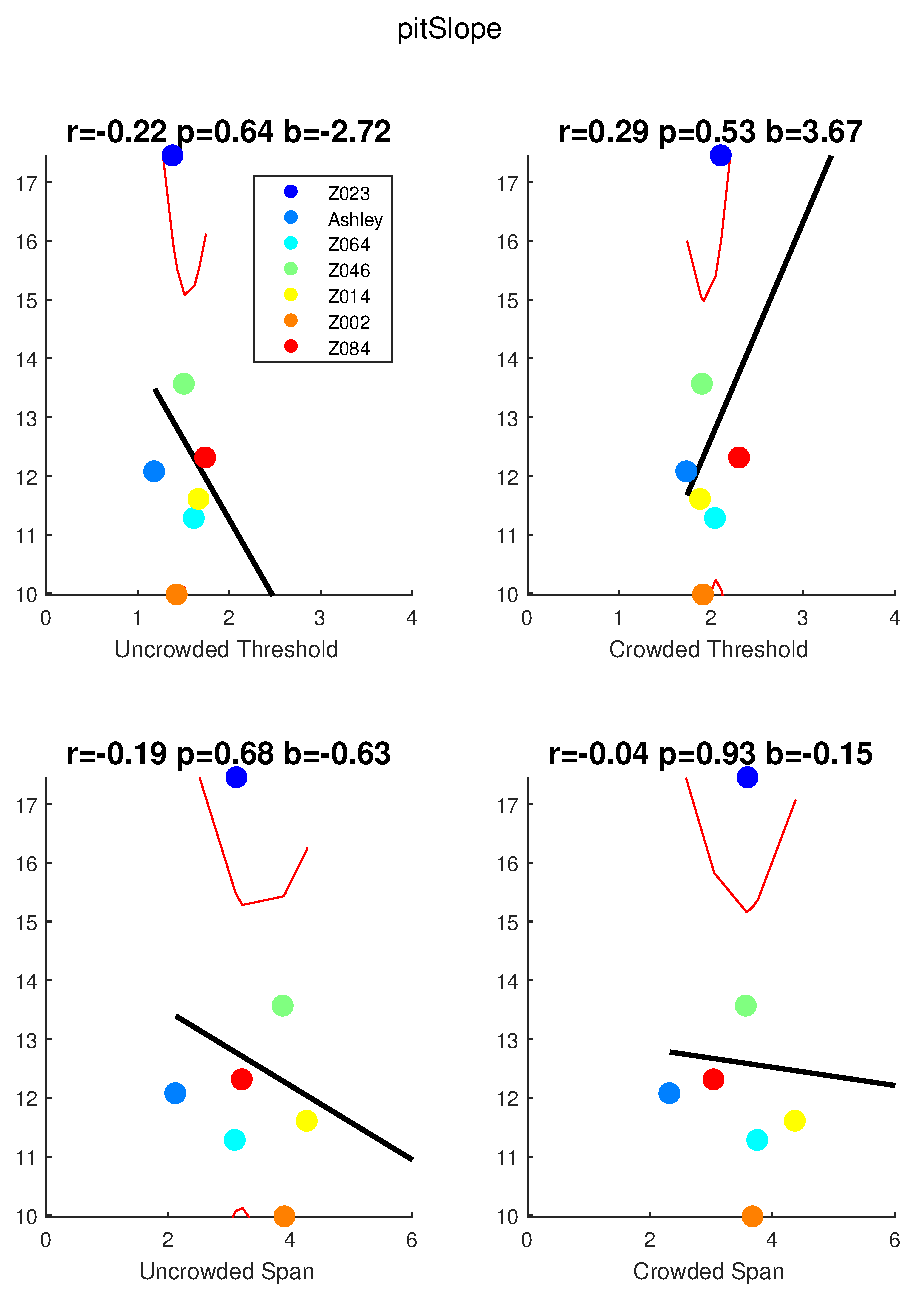
\includegraphics [width=4in]{runOCTAnalysis_03.eps}
	
	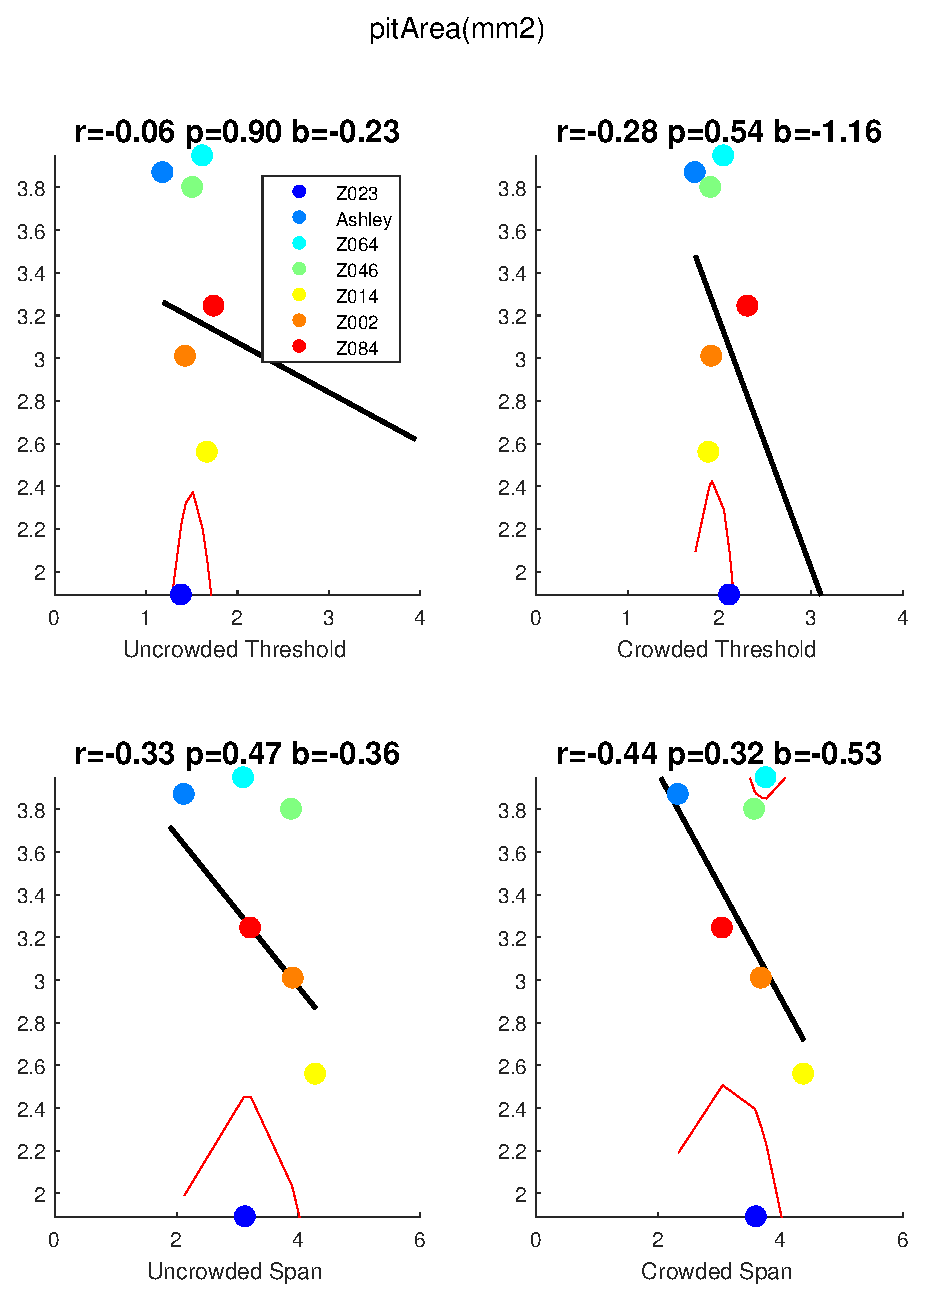
\includegraphics [width=4in]{runOCTAnalysis_04.eps}
	
	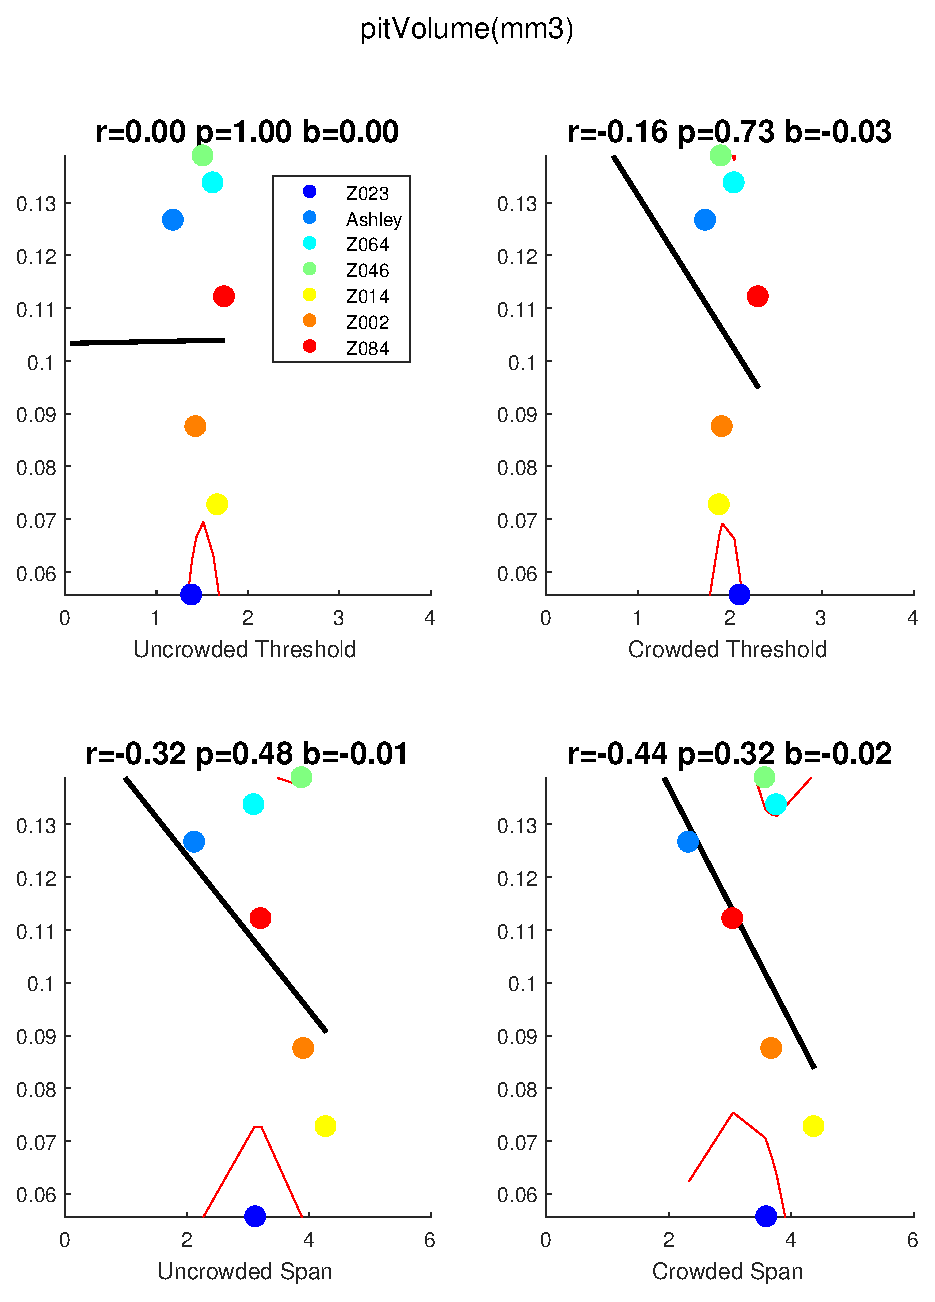
\includegraphics [width=4in]{runOCTAnalysis_05.eps}
	
	
	
\end{document}
    
